%& C:\Users\David\AppData\Roaming\TikzEdt\TikzEdt\021~1.0\TEMP_H~1
\begin{document}
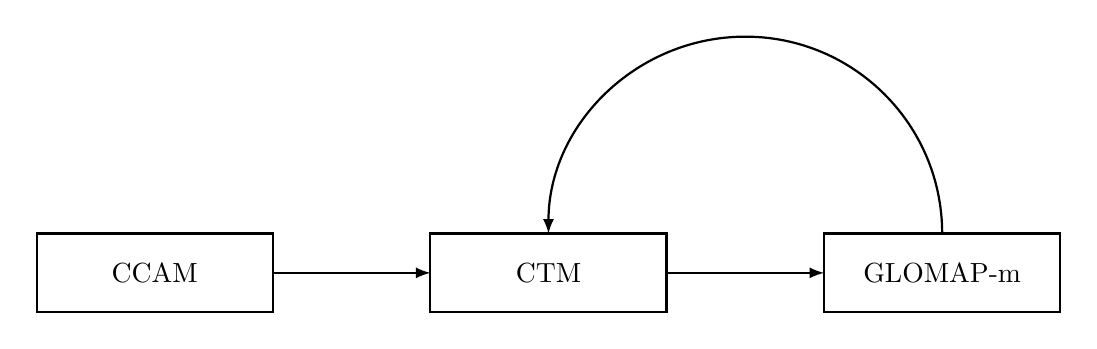
\begin{tikzpicture}

\draw[ thick]  (-1,1) rectangle (2,0) node[midway] {CCAM};
\draw[ thick]   (4,1) rectangle (7,0) node[midway] {CTM};
\draw[ thick]   (9,1) rectangle (12,0) node[midway] {GLOMAP-m};
\draw [-latex,  thick] (2,0.5) -- (4,0.5);
\draw[-latex,  thick] (7,0.5) -- (9,0.5);
\draw[-latex,  thick] (10.5,1) arc (-180:0:-2.5);

\usetikzlibrary{calc}
\pgftransformreset
\node[inner sep=0pt,outer sep=0pt,minimum size=0pt,line width=0pt,text width=0pt,text height=0pt] at (current bounding box) {};
%add border to avoid cropping by pdflibnet
\foreach \border in {0.1}
  \useasboundingbox (current bounding box.south west)+(-\border,-\border) rectangle (current bounding box.north east)+(\border,\border);
\newwrite\metadatafile
\immediate\openout\metadatafile=\jobname_BB.txt
\path
  let
    \p1=(current bounding box.south west),
    \p2=(current bounding box.north east)
  in
  node[inner sep=0pt,outer sep=0pt,minimum size=0pt,line width=0pt,text width=0pt,text height=0pt,draw=white] at (current bounding box) {
\immediate\write\metadatafile{\p1,\p2}
};
\immediate\closeout\metadatafile
\end{tikzpicture}

\end{document}
